\chapter{Réseau neuronal simple}

\section{Théorie}

\subsection{Le perceptron}

Le perceptron est le neurone le plus basique que l'on puisse trouver dans la littérature. Un perceptron est défini par : 
\begin{itemize}
\item $n$ entrées $x_i$
\item $1$ sortie $y$
\item $n$ poids $w_i$
\item $1$ biais $\theta$
\item $1$ fonction de composition $g : \mathbb{R}^n \to \mathbb{R}$
\item $1$ fonction d'activation $f : \mathbb{R} \to \mathbb{R}$
\end{itemize}

\vspace{\parskip}
Sur sa construction, le perceptron est fortement inspiré sur le neurone humain. Le perceptron détermine avec ses entrées si il "active" ou non la sortie, c'est à dire qu'il envoie un signal. Pour cela il rassemble toutes les données des entrées $x_i$ à l'aide de la fonction de composition $g$. Le neurone ne donnant pas la même importance à chaque entrée, on les pondère préalablement à l'aide des poids $w_i$. Finalement, on décide du signal de sortie à l'aide de la fonction d'activation $f$. De base, le seuil d'activation est souvent centrée en $0$. Pour palier à ce problème, on pondère l'entrée de la fonction d'activation par un biais $\theta$. En résumé, on a :

\[y = f(g(x_1w_1, x_2w_2, ... , x_nw_n) + \theta) \]

Usuellement, la fonction d'activation est la somme :

\[y = f(\sum_{i=1}^n x_iw_i + \theta) \]

On remarque que le biais agit comme le poids d'une entrée du neurone qui serait toujours $1$.

% \begin{figure}[!ht]
% \begin{center}
% \includegraphics[height=8cm]{simpleNeuron/Perceptron.png}
% \end{center}
% \caption{Schéma d'un perceptron standard\\Source Wikimedia Commons, sous license Creative Commons 3}
% \end{figure}

\subsection{Le réseau}

Une réseau de neurone permet de créer des fonctions de bien plus grande complexité qu'un simple neurone, permettant de résoudre des problèmes jusqu'alors inaccessible à la machine. Il permet par exemple de faire des prédictions sur le MNIST. Le MNIST est un problème où l'on a des images avec des chiffres écrit de manière manuscrites et l'on doit prédire le chiffre en question. C'est un problème d'une extrême simplicité pour un humain, mais un problème presque impossible pour une machine sans les réseaux de neurone. Ainsi pour construire un réseau, chaque perceptron est mis en relation avec ses pairs (un perceptron prend en entrée la sortie d'un autre perceptron). On construit alors un graphe orienté ou chaque sommet est un perceptron. On se limitera dans un premier temps au cas d'un réseau acyclique.

On peut définir plusieurs types de neurones dans un réseau:
\begin{itemize}
\item les neurones d'entrée
\item les neurones cachées
\item les neurones de sortie
\end{itemize}

\vspace{\parskip}
Il faut donc autant de neurones d'entrée que de dimensions qu'à l'échantillon que l'on veut soumettre au réseau. Par exemple dans le cadre du MNIST (insert cite here) on veut en entrée une image de dimension $28 \times 28$, on place donc $784$ neurones d'entrées. En pratique, les neurones d'entrée sont des neurones fictifs là pour faciliter la construction du réseau de neurone. En effet, il n'est pas soumis à un apprentissage et sa sortie est la même que son entrée. Nous ne les considérerons pas dans la théorie qui suit.

Les neurones des couches cachées sont présents entre les neurones d'entrée et de sortie. Ils sont utiles uniquement pour le calcul de la sortie. Le nombre de couches et la taille des couches influent sur l'action du réseau. Un réseau à multiples couches cachées sera capable de traiter des scénarios beaucoup plus complexes qu'un réseau à simple couche cachée. Cependant, cela augmente la complexité des calculs et le temps d'exécution.

Les neurones de sorties sont ceux qui servent pour la classification de l'échantillon d'entrée. Si l'on souhaite classifier une entrée il faut le même nombre de neurones de sortie que de classes différentes possibles. Ainsi dans l'exemple du MNIST, le but est de "deviner" un chiffre donné sur une image. Il y a donc $10$ possibilités (les 10 chiffres). Il y a donc $10$ neurones de sorties.

Dans toute la suite, on appellera $\{x_i\}_{i \leq n}$ les entrées, $\{y_i\}_{i \leq m}$ les sorties des neurones $\{y_i\}_{m+1-M \leq i \leq m}$ les sorties des neurones de sorties, $\{f_i\}_{i \leq m}$ les fonctions d'activations et $\{\theta_i\}_{i \leq m}$ les biais.

On définit enfin $\{F_i\}_{i \leq m}$ tel que $j \in E_i$ si et seulement si la sortie du neurone $j$ est reliée au neurone $i$. On peut ainsi numéroter les poids : $\{w_{ij}\}_{i \leq m, j \in F_i} $ le poids associé à l'entrée reliant le neurone $j$ au neurone $i$.

D'après ce qui précède, on obtient $\forall i \in [1, m]$ :

\[y_i = f_i(\sum_{j \in F_i} y_jw_{ij} + \theta_i) \]

\subsection{La rétropropagation}

L'efficacité d'un réseau de neurones se mesure à la qualité des prédictions qu'il est capable de faire. Cependant, il dépend des poids qui sont attribués à chaque entrée. Il faut donc déterminer la bonne combinaison de poids qui permettra au réseau de simuler la fonction voulu. Cependant, le nombre de poids présents dans un réseau augmente très rapidement et il devient très dur d'estimer cette bonne combinaison. Pour cela, on procède à un apprentissage : on utilise un échantillon de données dont on connaît le résultat pour construire un réseau avec les bon poids. On part ainsi d'un réseau avec des poids aléatoires, et on les modifie en prenant en compte les erreurs obtenus avec les échantillons d'apprentissage. Dans toute la suite, on s'intéressera à toute la démarche nécessaire pour arriver à cette modification de poids. On notera $\{x_i\}_{i \leq n}$ et $\{Y_i\}_{m+1-M \leq i \leq m}$ les entrées et sorties des échantillons.

Pour effectuer ces modifications, on calcule la sortie du réseau de neurone par un échantillon et on calcule l'erreur. Pour cela, on suppose que l'on possède une fonction $\epsilon : \mathbb{R}^2 \to \mathbb{R}^{+}$ qui mesure l'erreur entre deux nombres. L'erreur ainsi obtenue est :

\[ E = \sum_{i = m+1-M}^m \epsilon(y_i, Y_i)\]

On veut donc minimiser $E$ en modifiant les $w_{ij}$. Le problème ici est que l'on a une connaissance limitée de $E$ en fonction des $w_{ij}$ car l'on a les valeurs attendues que pour un nombre fini de valeur. Or les méthode de minimisation de fonction repose souvent sur une connaissance continue de ce que l'on veut optimiser. La seule méthode valable est la méthode des gradients.

Si l'on a une fonction $f$ que l'on veut minimiser par rapport à un facteur $x$. Alors on crée une suite $(x_n)$ tel que $x_{n+1} = x_{n} - \cfrac{\partial f}{\partial x}(x_n)$. L'idée est de modifier $x$ selon le gradient de la fonction à minimiser. Avec cette méthode, on peut calculer facilement la suite $(x_n)$ car l'on a besoin de calculer le gradient seulement en un point et non plus en un nombre continuement infini. Cependant, cette méthode est imprécise et il arrive qu'elle converge vers un minimum local de la fonction. En pratique, l'ajout de neurone va augmenter le nombre de dimension du gradient et donc permettre de limiter le nombre de minimum locaux.

On veut donc calculer pour tout $w_{ij}$ : $\cfrac{\partial E}{\partial w_{ij}}(w_{ij})$



\section{L'implémentation}

\subsection{Le neurone}

\subsection{Le réseau}

\subsection{La CLI}

\section{Bilan}

Après une semaine de débogage du code et de ses tests nous avons abouti à une solution fonctionnelle.

\subsection{Les résultats}

\subsection{Améliorations apportées}

Face à de tels temps de calcul, nous avons analysé la structure de notre code pour comprendre ce qui le ralentissait. De multiples causes majeures ont été identifiées : 
\begin{itemize}
\item La structure orientée objet
\item Le single-threading
\item calcul à chaque tour des sorties de chaque neurone
\end{itemize}

\bigskip

Nous nous sommes progressivement débarrassés de la structure d'objet du neurone en effectuant les conversions suivantes :

\bigskip

\begin{tabular}{c|c}
   structure objet & nouvelle structure \\
   \hline
   neurones.poids + matrice des poids + matrice des relations & matrice des poids \\
   neuron.activationFunction & vecteur de fonctions d'activation \\
   neuron.compositionFunction & on ne considère plus que la somme \\
   neuron.inputs/output & vecteur des entrées/sorties de tout le réseau \\
   neuron.bias & vecteur des biais de chaque neurone du réseau \\
   dérivée de la fonction de composition & vaut 1
\end{tabular}

\bigskip

De plus, nous avons déterminé en amont les neurones voisins qui nécessitaient un rafraîchissement de leur sortie. Cela permet de ne pas calculer à chaque itération la sortie de tous les neurones du réseau. Lors de la création du réseau, est construite une liste de vecteurs des neurones dont il faut évaluer la sortie au tour i.